%%%%%%%%%%%%%%%%%%%%%%% file template.tex %%%%%%%%%%%%%%%%%%%%%%%%%
%
% This is a general template file for the LaTeX package SVJour3
% for Springer journals.          Springer Heidelberg 2010/09/16
%
% Copy it to a new file with a new name and use it as the basis
% for your article. Delete % signs as needed.
%
% This template includes a few options for different layouts and
% content for various journals. Please consult a previous issue of
% your journal as needed.
%
%%%%%%%%%%%%%%%%%%%%%%%%%%%%%%%%%%%%%%%%%%%%%%%%%%%%%%%%%%%%%%%%%%%
%
% First comes an example EPS file -- just ignore it and
% proceed on the \documentclass line
% your LaTeX will extract the file if required
\begin{filecontents*}{example.eps}
%!PS-Adobe-3.0 EPSF-3.0
%%BoundingBox: 19 19 221 221
%%CreationDate: Mon Sep 29 1997
%%Creator: programmed by hand (JK)
%%EndComments
gsave
newpath
  20 20 moveto
  20 220 lineto
  220 220 lineto
  220 20 lineto
closepath
2 setlinewidth
gsave
  .4 setgray fill
grestore
stroke
grestore
\end{filecontents*}
%
\RequirePackage{fix-cm}
%
%\documentclass{svjour3}                     % onecolumn (standard format)
%\documentclass[smallcondensed]{svjour3}     % onecolumn (ditto)
\documentclass[smallextended, natbib]{svjour3}       % onecolumn (second format)
%\documentclass[twocolumn]{svjour3}          % twocolumn
%
\smartqed  % flush right qed marks, e.g. at end of proof
%
\usepackage{graphicx}
\usepackage{tikz}

%
 \usepackage{mathptmx}      % use Times fonts if available on your TeX system
%
% insert here the call for the packages your document requires
\usepackage{amsmath}
\usepackage{gensymb}
%\usepackage{latexsym}
% etc.
%
% please place your own definitions here and don't use \def but
% \newcommand{}{}
%
% Insert the name of "your journal" with
% \journalname{myjournal}
%
\begin{document}

\title{The Furuta Pendulum
%\thanks{Grants or other notes
%about the article that should go on the front page should be
%placed here. General acknowledgments should be placed at the end of the article.}
}
\subtitle{Technical Report}

%\titlerunning{Short form of title}        % if too long for running head

\author{Tabea A. Wilke \and Yannik P. Frisch \and \\Maximilian A. Gehrke
}

%\authorrunning{Wilke, Gehrke, Frisch} % if too long for running head

\institute{Tabea A. Wilke \at
	TU Darmstadt, Germany\\
	\email{tabeaalina.wilke@stud.tu-darmstadt.de}           %  \\
	%             \emph{Present address:} of F. Author  %  if needed
	\and
	Yannik P. Frisch \at
	TU Darmstadt, Germany\\
	\email{yannik\_phil.frisch@stud.tu-darmstadt.de}
	\and
	Maximilian A. Gehrke \at
	TU Darmstadt, Germany\\
	\email{maximilian\_alexander.gehrke@stud.tu-darmstadt.de}
}

\date{Received: date / Accepted: date}
% The correct dates will be entered by the editor


\maketitle

\begin{abstract}
The Furuta Pendulum is a complex non-linear system and therefore 
of big interest in control system theory. It consists of one controllable arm 
rotating in the horizontal plane and one pendulum, which is attached to the end 
of this arm, moving uncontrollably in the vertical plane.\\
The non-linearities result from an interplay between gravitational, coriolis, 
centrifugal forces and friction. They can be modeled through equations of 
motion through the Euler-Lagrange method.\\
We present an overview over its technical details and discuss algorithms to 
solve the control problem.
\keywords{Furuta Pendulum \and Reinforcement Learning \and Equations of 
motion}
% \PACS{PACS code1 \and PACS code2 \and more}
% \subclass{MSC code1 \and MSC code2 \and more}
\end{abstract}
\section{Introduction}
Many examples in the field of control engineering like aircraft landing or 
aircraft stabilizing can be well modeled by an inverted 
pendulum \citep{akhtaruzzaman2010modeling}. As a reaction to problems with the 
limited movement of the cart from 
the inverted pendulum, the Furuta pendulum (also called rotary inverted 
pendulum) 
has been developed by 
\cite{furuta1992swing}. The advantages of the Furuta pendulum are that 
it 
needs less space and one moving arm is directly linked to the motor. Therefore, 
the dynamics is less unmodeled thanks to a power transmission mechanism 
\citep{furuta1992swing}. \\
The Furuta pendulum is an underactuated system. An underactuated system is 
characterized by the difference of the degrees of freedom and the number of 
actuators. If there are more degrees of freedom, the system is trivially 
underactuated \citep{tedrake2009underactuated}.Therefore, it is not possible to 
accelerate the system in every direction. In case of the Furuta pendulum, this 
means that there are two degrees of freedom ($\phi,\ \theta$), 
but only one arm is directly controlled by the motor. This is the one which 
changes the angle $\phi$ in the horizontal plane. The other arm, called 
pendulum, 
is attached to 
the end of the controlled arm and therefore is moved indirectly by it in the 
vertical plane with angle $\theta$ 
\citep{spong1998underactuated,tedrake2009underactuated}. The whole system is 
highly non-linear as a result of an interplay between gravitational, coriolis, 
friction and centrifugal forces \citep{izutsu2008swing}.
\begin{figure}[h]
	\centering
	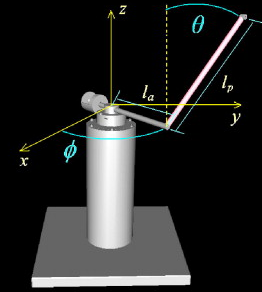
\includegraphics[width=0.5\linewidth]{pendulum}
	\caption{A typical structure of the Furuta pendulum with the most important 
	variables, figure from \cite{la2009new}.}
	\label{fig:pendulum}
\end{figure}\\
Finally, there are two different types of control problems, "swing-up" and 
"stabilization". The swing-up task consists in bringing the 
flexible arm from a hanging position to a position which is nearly upright. 
Stabilization considers the problem when the arm is nearly upright with low 
enough speed, balancing it to hold this state stable. 
\subsection{Definitions}
The system (see Fig. \ref{fig:pendulum}) consists of an arm with length $l_a$ 
mounted to a DC motor, which is 
able to apply a torque $\tau$ to it. It has a mass of $m_a$. Another arm with 
length $l_p$ and mass 
$m_p$
is attached to the remaining side of the 
first arm. Both arms have a moment of inertia $J_a$ and $J_p$ respectively. The 
counter force to the input torque is the viscous damping $B_a$ because of the 
bearings of the motor. As the pendulum is not controlled directly, the only 
force that is directly applied to the pendulum is damping at the connection to 
the arm $B_p$. The angles are given in radian, where an angle $\theta$ of zero 
refers to the upright position.

\section{Mathematical Modelling} 
The kinematics of the pendulum's 
center of gravity can be described by 
\[\mathbf{p_{cg}}=\begin{bmatrix}
x	\\ 
y	\\ 
z	
	\end{bmatrix} =\begin{bmatrix}
l_a\cos\phi-l_{p}\sin\theta\sin\phi \\ 
l_a\sin\phi+l_{p}\sin\theta\cos\phi \\ 
l_{p}\cos\theta
\end{bmatrix}. \] 
The relative velocity of the pendulum to the arm can be represented by 
\[\mathbf{v_{cg}}= \begin{bmatrix}
\dot{x}\\
\dot{y}\\
\dot{z}\end{bmatrix}=\begin{bmatrix}
-l_a\ \sin \phi \dot{\phi}-l_{p}\ \cos\phi \sin\theta\dot{\phi}-l_{p} 
\ \sin\phi \cos\theta\dot{\theta} \\ 
l_a\ \cos\phi\dot{\phi}-l_{p} \ \sin\phi \sin\theta\dot{\phi}+l_{p} 
\ \cos\theta \cos\phi\dot{\theta} \\
-l_{p} \ \sin\theta\dot{\theta}
\end{bmatrix}.\]
The equations of motion can be derived through the Euler-Lagrange 
method. The Lagrangian function is given by the difference of the 
kinetic and potential energies $L=T-V$, with $T$ as the total sum of the 
kinetic energies in the system and $V$ the total potential energies.\\
The only potential energy in the system is the one of the pendulum:
\[V_{total}=V_{pendulum}=m_pgz= m_pgl_{p}\cos\theta.\]
Kinetic energy is available both in the arm and in the pendulum and is composed 
of the sum of translation energy and rotational energy. The translation 
energy $T=\frac{1}{2}mv^2$ uses the squared velocity. This is defined by  the 
scalar product 
of the squared velocities in all directions:
\begin{align*}v^2&=\dot{x}^2+\dot{y}^2+\dot{z}^2\\
&=(l_a^2+l_p^2\ 
\sin^2\theta)\dot{\phi}^2+l_p^2\dot{\theta}^2+2l_al_p\dot{\phi}\dot{\theta}\cos 
\theta\end{align*} 
\begin{align*}
T_{arm}&=\frac{1}{2}J_a\dot{\phi}^2\\
T_{pendulum}&=\frac{1}{2}J_p\dot{\theta}^2+\frac{1}{2}m_pv^2\\
&= \frac{1}{2}J_p\dot{\theta}^2+\frac{1}{2}m_p\left((l_a^2+l_p^2\ 
\sin^2\theta)\dot{\phi}^2+l_p^2\dot{\theta}^2+2l_al_p\dot{\phi}\dot{\theta}\cos 
\theta\right)\\
T_{total}&= 
\frac{1}{2}J_a\dot{\phi}^2+\frac{1}{2}J_p\dot{\theta_0}^2+\frac{1}{2}m_p\left((l_a^2+l_p^2\
\sin^2\theta)\dot{\phi}^2+l_p^2\dot{\theta}^2+2l_al_p\dot{\phi}\dot{\theta}\cos 
\theta\right).
\end{align*}
From this the Lagrange Function arises:
\begin{align*}
L &=T_{total}-V_{total}\\
\begin{split}&=\frac{1}{2}J_a\dot{\phi}^2+\frac{1}{2}J_p\dot{\theta}^2+\frac{1}{2}m_p\left((l_a^2+l_p^2\
\sin^2\theta)\dot{\phi}^2+l_p^2\dot{\theta}^2+2l_al_p\dot{\phi}\dot{\theta}\cos 
\theta\right) \\&\quad - m_pgl_{p}\cos\theta.\end{split}
\end{align*}
 Lagrange's 
Equation follows \[ 
\frac{d}{dt}\left(\frac{\partial L(q, \dot{q},t)}{\partial 
	\dot{q_i}}\right)-\frac{\partial 
	L(q, \dot{q},t)}{\partial 
	q_i}+\frac{\partial F(q, \dot{q}, t)}{\partial \dot{q_i}} =0.\] Thereby, 
	the 
	variables 
	$q_i$ are called 
	generalized coordinates. $F$ is the friction in 
	the system, which can be described with the damping coefficients 
	$(B_a, B_p)$ by $B_p\dot{\theta}$ and $ 
	B_a\dot{\phi}$.
	For 
the Furuta pendulum the generalized coordinates are $q(t)^T=[\phi \ \theta]$ 
with 
the derivation according to time $\dot{q}(t)^T = 
\left[\frac{\partial 
	\phi(t)}{\partial t}\ \frac{\partial \theta(t)}{\partial t} \right]$. 
	Together, this
	leads 
to 
\begin{align}
\frac{\partial^2 L}{\partial t\partial \dot{\phi}}-\frac{\partial 
	L}{\partial \phi}&=\tau - B_a\dot{\phi} \label{eq:f1}\\
\frac{\partial^2 L}{\partial t\partial \dot{\theta}}-\frac{\partial 
	L}{\partial \theta}&=-B_p\dot{\theta}\label{eq:f2}.
\end{align}
The partial derivations of the Lagrangian for the generalized coordinates are:

\begin{align*}
	\frac{\partial L}{\partial \phi}&=0\\
	\frac{\partial L}{\partial 
	\dot{\phi}}&=\dot{\phi}(J_a+m_p(l_a^2+l_p^2\sin^2\theta))+\dot{\theta}(
	m_pl_al_p\cos\theta)\\
	\frac{\partial^2 L}{\partial t \partial \dot{\phi}}&= 
	\ddot{\phi}(J_a+m_p(l_a^2+l_p^2\sin^2 \theta))+l_p^2m_p\sin(2\theta)
	\dot{\phi}\dot{\theta}+m_pl_al_p(\cos 
	\theta\ddot{\theta}-sin\theta \dot{\theta}^2)\\
	\frac{\partial L}{\partial 
	\theta}&=\frac{1}{2}\dot{\phi}^2m_pl_p^2\sin(2\theta)-m_pl_al_psin\theta\dot{\phi}
	\dot{\theta}+m_pgl_psin\theta\\
	\frac{\partial L}{\partial 
		\dot{\theta}}&=\dot{\theta}(J_p+m_pl_p^2)+\dot{\phi}(m_pl_al_p\cos\theta)\\
	\frac{\partial^2 L}{\partial t \partial 
	\dot{\theta}}&=\ddot{\theta}(J_p+m_pl_p^2)+\ddot{\phi}m_pl_al_p\cos\theta-\dot{\phi}
	\dot{\theta}m_pl_al_p\sin\theta.
\end{align*}
With this equations it is possible to derive the equations for the 
Euler-Lagrange's Equation:
\begin{align*}
\frac{\partial^2 L}{\partial t\partial\dot{\phi}}-\frac{\partial 
L}{\partial\dot{\phi}}&=\ddot{\phi}(J_a+m_p(l_a^2+l_p^2\sin^2 
\theta))+l_p^2m_p\sin(2\theta)
\dot{\phi}\dot{\theta}\\ &\quad + m_pl_al_p(\cos 
\theta\ddot{\theta}-sin\theta \dot{\theta}^2)\\
\frac{\partial^2 L}{\partial t\partial\dot{\theta}}-\frac{\partial 
L}{\partial\dot{\theta}}&=\ddot{\theta}(J_p+m_pl_p^2)+\ddot{\phi}m_pl_al_p\cos\theta-\frac{1}{2}\dot{\phi}^2m_pl_p^2\sin(2\theta)-m_pgl_psin\theta
.\end{align*}
Putting this into a matrix form and filling in the friction, this results in 
the nonlinear equations of motion (EOM) for the Furuta pendulum:
\begin{align*}
&\begin{bmatrix}
J_a+m_p(l_a^2+l_p^2\sin^2\theta)& \quad m_pl_al_p\cos\theta \\ 
m_pl_al_p\cos\theta& \quad J_p+m_pl_p^2 
\end{bmatrix} 
\begin{bmatrix}
\ddot{\phi}\\
\ddot{\theta}
\end{bmatrix} + \\
&\begin{bmatrix}
m_pl_p^2\sin(2\theta)\dot{\theta}+ B_a& \quad -m_pl_al_p\sin \theta 
\dot{\theta}\\
-\frac{1}{2}m_pl_p^2\sin(2\theta)\dot{\phi} &\quad B_p
\end{bmatrix}
\begin{bmatrix}
\dot{\phi}\\
\dot{\theta}
\end{bmatrix} +
\begin{bmatrix}
0\\
-m_pl_pg\sin\theta
\end{bmatrix}=\begin{bmatrix}
\tau \\
0
\end{bmatrix}.
\end{align*}
\subsection{Linearization of the State-Space Model}
As all equations of motion contain a part of a trigonometric function, the 
equations are non-linear. There are several different methods to transform the 
non-linear equations to linear ones, for example Taylor expansion with 
substituting non-linear parts \citep{hamza2015genetic}, Jacobian 
linearization \citep{al2013experimental} or optimal linearization 
\citep{zhang2011optimal}.
 For a linearization in the state-space the equation 
$\dot{x}=Ax+Bu$ with $x=[\phi\ \theta\ \dot{\phi}\ \dot{\theta}]$ is used. The 
linearization is done around the 
operating point \citep{furuta1992swing}, which is the vertical inverted 
state and, therefore, uses $x_0=[0 \ 0\ 0\ 0]^T$. This results in 
the following equations: 
\begin{align}
\dot{x}=
\begin{bmatrix}
0	& 0 &1  &0  \\ 
0	&  0& 0 &  1\\ 
\frac{\partial f_1(x,\tau)}{\partial \phi}\Big|_{x=x_0}	& \frac{\partial 
f_1(x,\tau)}{\partial \theta}\Big|_{x=x_0} & \frac{\partial 
f_1(x,\tau)}{\partial 
\dot{\phi}}\Big|_{x=x_0} & \frac{\partial f_1(x,\tau)}{\partial 
\dot{\theta}}\Big|_{x=x_0} \\ 
\frac{\partial f_2(x,\tau)}{\partial \phi}\Big|_{x=x_0}	& \frac{\partial 
	f_2(x,\tau)}{\partial \theta}\Big|_{x=x_0} & \frac{\partial 
	f_2(x,\tau)}{\partial 
	\dot{\phi}}\Big|_{x=x_0} & \frac{\partial f_2(x,\tau)}{\partial 
	\dot{\theta}}\Big|_{x=x_0} 
\end{bmatrix} 
x +
\begin{bmatrix}
0	\\ 
0	\\ 
\frac{\partial f_1(x,\tau)}{\partial 
	\tau}\Big|_{x=x_0} 	\\
\frac{\partial f_2(x,\tau)}{\partial 
	\tau}\Big|_{x=x_0} 
\end{bmatrix} \tau
\label{eq:liner}
\end{align} with $f_1$ as Eq. \eqref{eq:f1} and $f_2$ as Eq. \eqref{eq:f2}.\\
The result is a linear form of the equations of motion which are very close to 
the system's description by the non-linear model. For an angle of 
$\theta<25\degree$  
there is nearly no discrepancy to the actual motion
which \cite{kurode2011swing} showed.

\section{Pendulum Control}
The goal of controlling the Furuta pendulum is to bring it from a hanging 
position into a vertical upright position. Therefore, it is necessary to 
generate enough energy to swing the pendulum up in a nearly upright position 
where the linear region begins \citep{kurode2011swing}. If this region is 
reached, the controller should change to the balancing mode to stabilize the 
upright position.\\
To check whether the controller needs to be switched from the swing-up task to 
the stabilize task, the switching criteria can for 
example be defined by \citep{hamza2019current}:
\begin{align*}
\text{switching criteria}
\begin{cases} \text{stabilization} &\begin{cases}
|\theta|< \frac{\pi}{9} \ &\text{and}\  \dot{\theta} < 2.62\  \text{rad/sec}\\
|E-E_r|< 0.04 \ \text{Joule}\ &\text{and}\  \dot{\theta} < 2.62\  \text{rad/sec}
\end{cases}\\
\text{swing-up} & \text{otherwise}
\end{cases}.
\end{align*}
\subsection{Swing-Up}
There are many different approaches for solving the swing-up task of the Furuta 
pendulum: linear ones which use the linearized equations of motion, non-linear 
ones and model-free approaches. The classical way of solving the swing-up task 
is 
an approach with energy control \citep{seman2013swinging}. Therefore, the sum 
of 
kinetic and potential energy of the pendulum is used to model which amount of 
energy should be added. The energy of the pendulum can be described by 
\[E = \frac{1}{2}J_p\theta^2+m_pgl_p(\cos \theta -1),\] which was already done 
by \cite{aastrom2000swinging} for the normal pendulum.
As we want to stabilize the pendulum on an upright position, optimally we do 
not need any further energy in this state. Therefore, this is a logical state 
to set as state without any energy left \citep{seman2013swinging}.\\
There are two different directions in which the 
energy can be supplied. Either the pendulum seems to be "pulled" or "pushed" 
\cite{seman2013swinging}. Therefore, we need a sign-function that represents 
whether to push or pull. The argument of the sign-function is compound by the 
velocity which specifies whether the pendulum starts to swing in the opposite 
direction and a cosine that defines the side of the pendulum. This results in 
the term, $\text{sign}(\dot{\theta}\cos\theta)$ 
\citep{awtar2002inverted}. \\
The magnitude of energy which should be provided is 
selected by an aggressivity factor and the difference of actual and desired 
system energy $k_a(E-E_0)$, with $E_0=0$ as the system should have zero energy 
at the end. The aggressivity factor handles the amount of input 
and thereby the number of oscillations which are needed to achieve the 
swing-up \citep{awtar2002inverted}. Often there is also a saturation function 
which 
limits the signal to the maximum acceleration of the pendulum. This is done 
with a linear function, in the following described as a wildcard $sat$. The 
whole 
swing-up controller is then implemented by 
\begin{align*}
u = sat(k_a(E-E_0))\text{sign}(\dot{\theta}\cos\theta).
\end{align*}
\subsection{Stabilization}
There are many different approaches for solving the stabilization problem as 
well. The most common one is the linear quadratic regulation (LQR) because it 
guarantees the optimal solution \citep{hamza2019current}. Also the 
proportional integral derivative (PID) is often used because of its simplicity 
and robustness and also because of its usage in industry 
\citep{hassanzadeh2011controller}. Nevertheless, there are a lot of other 
algorithms from sliding modes \citep{izutsu2008swing} to particle swarm 
optimization and other evolutionary algorithms 
\citep{hassanzadeh2011controller}.\\
In the following, we will shortly describe how an LQR controller can be modeled 
for the stabilization problem on the Furuta Pendulum. The LQR is a controller 
which can be used to make a controllable, but unstable system stable 
\citep{park2011swing}. It uses the linearized equations of motion in the 
state-space model in form of a state feedback method \citep{ozbek2010swing}. 
The cost function can be defined with $x=[\phi \ \theta \ \dot{\phi}\ 
\dot{\theta}]^T$, $R$ and $Q$ as weighting matrix by 
\citep{al2013experimental},
\[J=\int_{0}^{\infty}\left(x^TQx+u^TRu\right)\text{d}t.\]
The constraint for the cost function is the systems dynamic in form of a 
differential equation derived from the linearization $\dot{x}=Ax+Bu$, see 
Eq. \eqref{eq:liner}. To solve 
the cost function linear state feedback with a constant gain matrix $K$ is 
used: $u(t)=-Kx(t)$ with $K=-R^{-1}B^TP$. $P(t)$ is the 
solution matrix which will stabilize ($\dot{P}(t)=0$) for a convergent system 
\citep{chen2007linear}. It 
is a symmetric matrix which holds the algebraic Riccati equation (ARE) 
\citep{al2013experimental}
\[PA+A^TP-PBR^{-1}B^TP+Q=0.\]

\section{Reinforcement Learning on the Furuta Pendulum}
In reinforcement learning, the Furuta pendulum has only a very small influence 
on research maybe also because of the complexity of the 
problem. Only a few algorithms were tested on it with divers results. 
Reinforcement learning should play a bigger role in solving the Furuta pendulum 
because it could improve the robustness of the stabilization control 
\citep{wang2004minimum}.\\
\cite{hennig2011optimal} compares Gaussian process optimal learner with 
Kalman filter, TD($\lambda$) and full information as baseline. He used the same 
baseline function for all algorithms and collated the cumulated loss. 
Surprisingly, none of the methods could stabilize the swung up pendulum 
totally, even not the best method, the Gaussian process optimal learner.\\
An artificial neural network (ANN) was used to model the pendulum 
\citep{quyen2012rotary}. They worked with the voltage of the motor as input 
values and the angles of arm and pendulum as the output. They used a PID 
controller for a supervised training. Different numbers of 
hidden neurons were tested with the result that more neurons in the hidden 
layer led to a smaller mean squared error. The ANN could predict the angle of 
the pendulum very well.\\
Another approach to stabilize the pendulum was done with recurrent neural 
networks (RNN) and a Genetic Algorithm 
\citep{shojaei2011hybrid}. They used a recurrent neural network identifier and 
controller with a proportional integral derivative controller, which was 
responsible for the feedback and the prediction. The RNN identifier checks 
whether the output of the feedback system is valid or not. The RNN controller 
handles the power of the system.\\
The "Application of Reinforcement Learning Methods" course of the TU Darmstadt 
implemented different reinforcement learning algorithms on different platforms. 
Some of the algorithms were also tested on the qube simulation of the Quanser 
system, which is identical to the Furuta pendulum. The maximum reward per 
episode was 6.0 with an maximum episode length of 300 steps. The results can be 
found in Fig. \ref{fig:rewards} with a simulation evaluation of 100 episodes. 
None of the different algorithms clearly outperform the others. They have very 
similar results.\\
Further on, two groups managed to run their algorithm on the real Qube Quanser 
robot platform and received 4.88 (PPO, 25 evaluated episodes) and 4.2 (DQN, 10 
evaluated episodes) out of 6.0 possible rewards.  

 \begin{figure}[h]
 	\centering
	\scalebox{.4}{%% Creator: Matplotlib, PGF backend
%%
%% To include the figure in your LaTeX document, write
%%   \input{<filename>.pgf}
%%
%% Make sure the required packages are loaded in your preamble
%%   \usepackage{pgf}
%%
%% Figures using additional raster images can only be included by \input if
%% they are in the same directory as the main LaTeX file. For loading figures
%% from other directories you can use the `import` package
%%   \usepackage{import}
%% and then include the figures with
%%   \import{<path to file>}{<filename>.pgf}
%%
%% Matplotlib used the following preamble
%%   \usepackage{fontspec}
%%   \setmainfont{DejaVuSerif.ttf}[Path=/home/tabea/.conda/envs/rl-hw1/lib/python3.6/site-packages/matplotlib/mpl-data/fonts/ttf/]
%%   \setsansfont{DejaVuSans.ttf}[Path=/home/tabea/.conda/envs/rl-hw1/lib/python3.6/site-packages/matplotlib/mpl-data/fonts/ttf/]
%%   \setmonofont{DejaVuSansMono.ttf}[Path=/home/tabea/.conda/envs/rl-hw1/lib/python3.6/site-packages/matplotlib/mpl-data/fonts/ttf/]
%%
\begingroup%
\makeatletter%
\begin{pgfpicture}%
\pgfpathrectangle{\pgfpointorigin}{\pgfqpoint{6.400000in}{4.800000in}}%
\pgfusepath{use as bounding box, clip}%
\begin{pgfscope}%
\pgfsetbuttcap%
\pgfsetmiterjoin%
\definecolor{currentfill}{rgb}{1.000000,1.000000,1.000000}%
\pgfsetfillcolor{currentfill}%
\pgfsetlinewidth{0.000000pt}%
\definecolor{currentstroke}{rgb}{1.000000,1.000000,1.000000}%
\pgfsetstrokecolor{currentstroke}%
\pgfsetdash{}{0pt}%
\pgfpathmoveto{\pgfqpoint{0.000000in}{0.000000in}}%
\pgfpathlineto{\pgfqpoint{6.400000in}{0.000000in}}%
\pgfpathlineto{\pgfqpoint{6.400000in}{4.800000in}}%
\pgfpathlineto{\pgfqpoint{0.000000in}{4.800000in}}%
\pgfpathclose%
\pgfusepath{fill}%
\end{pgfscope}%
\begin{pgfscope}%
\pgfsetbuttcap%
\pgfsetmiterjoin%
\definecolor{currentfill}{rgb}{1.000000,1.000000,1.000000}%
\pgfsetfillcolor{currentfill}%
\pgfsetlinewidth{0.000000pt}%
\definecolor{currentstroke}{rgb}{0.000000,0.000000,0.000000}%
\pgfsetstrokecolor{currentstroke}%
\pgfsetstrokeopacity{0.000000}%
\pgfsetdash{}{0pt}%
\pgfpathmoveto{\pgfqpoint{0.800000in}{0.528000in}}%
\pgfpathlineto{\pgfqpoint{5.760000in}{0.528000in}}%
\pgfpathlineto{\pgfqpoint{5.760000in}{4.224000in}}%
\pgfpathlineto{\pgfqpoint{0.800000in}{4.224000in}}%
\pgfpathclose%
\pgfusepath{fill}%
\end{pgfscope}%
\begin{pgfscope}%
\pgfpathrectangle{\pgfqpoint{0.800000in}{0.528000in}}{\pgfqpoint{4.960000in}{3.696000in}}%
\pgfusepath{clip}%
\pgfsetbuttcap%
\pgfsetmiterjoin%
\definecolor{currentfill}{rgb}{0.194608,0.453431,0.632843}%
\pgfsetfillcolor{currentfill}%
\pgfsetlinewidth{0.000000pt}%
\definecolor{currentstroke}{rgb}{0.000000,0.000000,0.000000}%
\pgfsetstrokecolor{currentstroke}%
\pgfsetstrokeopacity{0.000000}%
\pgfsetdash{}{0pt}%
\pgfpathmoveto{\pgfqpoint{0.899200in}{0.528000in}}%
\pgfpathlineto{\pgfqpoint{1.692800in}{0.528000in}}%
\pgfpathlineto{\pgfqpoint{1.692800in}{4.048000in}}%
\pgfpathlineto{\pgfqpoint{0.899200in}{4.048000in}}%
\pgfpathclose%
\pgfusepath{fill}%
\end{pgfscope}%
\begin{pgfscope}%
\pgfpathrectangle{\pgfqpoint{0.800000in}{0.528000in}}{\pgfqpoint{4.960000in}{3.696000in}}%
\pgfusepath{clip}%
\pgfsetbuttcap%
\pgfsetmiterjoin%
\definecolor{currentfill}{rgb}{0.881863,0.505392,0.173039}%
\pgfsetfillcolor{currentfill}%
\pgfsetlinewidth{0.000000pt}%
\definecolor{currentstroke}{rgb}{0.000000,0.000000,0.000000}%
\pgfsetstrokecolor{currentstroke}%
\pgfsetstrokeopacity{0.000000}%
\pgfsetdash{}{0pt}%
\pgfpathmoveto{\pgfqpoint{1.891200in}{0.528000in}}%
\pgfpathlineto{\pgfqpoint{2.684800in}{0.528000in}}%
\pgfpathlineto{\pgfqpoint{2.684800in}{3.809936in}}%
\pgfpathlineto{\pgfqpoint{1.891200in}{3.809936in}}%
\pgfpathclose%
\pgfusepath{fill}%
\end{pgfscope}%
\begin{pgfscope}%
\pgfpathrectangle{\pgfqpoint{0.800000in}{0.528000in}}{\pgfqpoint{4.960000in}{3.696000in}}%
\pgfusepath{clip}%
\pgfsetbuttcap%
\pgfsetmiterjoin%
\definecolor{currentfill}{rgb}{0.229412,0.570588,0.229412}%
\pgfsetfillcolor{currentfill}%
\pgfsetlinewidth{0.000000pt}%
\definecolor{currentstroke}{rgb}{0.000000,0.000000,0.000000}%
\pgfsetstrokecolor{currentstroke}%
\pgfsetstrokeopacity{0.000000}%
\pgfsetdash{}{0pt}%
\pgfpathmoveto{\pgfqpoint{2.883200in}{0.528000in}}%
\pgfpathlineto{\pgfqpoint{3.676800in}{0.528000in}}%
\pgfpathlineto{\pgfqpoint{3.676800in}{4.019346in}}%
\pgfpathlineto{\pgfqpoint{2.883200in}{4.019346in}}%
\pgfpathclose%
\pgfusepath{fill}%
\end{pgfscope}%
\begin{pgfscope}%
\pgfpathrectangle{\pgfqpoint{0.800000in}{0.528000in}}{\pgfqpoint{4.960000in}{3.696000in}}%
\pgfusepath{clip}%
\pgfsetbuttcap%
\pgfsetmiterjoin%
\definecolor{currentfill}{rgb}{0.753431,0.238725,0.241667}%
\pgfsetfillcolor{currentfill}%
\pgfsetlinewidth{0.000000pt}%
\definecolor{currentstroke}{rgb}{0.000000,0.000000,0.000000}%
\pgfsetstrokecolor{currentstroke}%
\pgfsetstrokeopacity{0.000000}%
\pgfsetdash{}{0pt}%
\pgfpathmoveto{\pgfqpoint{3.875200in}{0.528000in}}%
\pgfpathlineto{\pgfqpoint{4.668800in}{0.528000in}}%
\pgfpathlineto{\pgfqpoint{4.668800in}{3.622435in}}%
\pgfpathlineto{\pgfqpoint{3.875200in}{3.622435in}}%
\pgfpathclose%
\pgfusepath{fill}%
\end{pgfscope}%
\begin{pgfscope}%
\pgfpathrectangle{\pgfqpoint{0.800000in}{0.528000in}}{\pgfqpoint{4.960000in}{3.696000in}}%
\pgfusepath{clip}%
\pgfsetbuttcap%
\pgfsetmiterjoin%
\definecolor{currentfill}{rgb}{0.578431,0.446078,0.699020}%
\pgfsetfillcolor{currentfill}%
\pgfsetlinewidth{0.000000pt}%
\definecolor{currentstroke}{rgb}{0.000000,0.000000,0.000000}%
\pgfsetstrokecolor{currentstroke}%
\pgfsetstrokeopacity{0.000000}%
\pgfsetdash{}{0pt}%
\pgfpathmoveto{\pgfqpoint{4.867200in}{0.528000in}}%
\pgfpathlineto{\pgfqpoint{5.660800in}{0.528000in}}%
\pgfpathlineto{\pgfqpoint{5.660800in}{3.761525in}}%
\pgfpathlineto{\pgfqpoint{4.867200in}{3.761525in}}%
\pgfpathclose%
\pgfusepath{fill}%
\end{pgfscope}%
\begin{pgfscope}%
\pgfsetbuttcap%
\pgfsetroundjoin%
\definecolor{currentfill}{rgb}{0.000000,0.000000,0.000000}%
\pgfsetfillcolor{currentfill}%
\pgfsetlinewidth{0.803000pt}%
\definecolor{currentstroke}{rgb}{0.000000,0.000000,0.000000}%
\pgfsetstrokecolor{currentstroke}%
\pgfsetdash{}{0pt}%
\pgfsys@defobject{currentmarker}{\pgfqpoint{0.000000in}{-0.048611in}}{\pgfqpoint{0.000000in}{0.000000in}}{%
\pgfpathmoveto{\pgfqpoint{0.000000in}{0.000000in}}%
\pgfpathlineto{\pgfqpoint{0.000000in}{-0.048611in}}%
\pgfusepath{stroke,fill}%
}%
\begin{pgfscope}%
\pgfsys@transformshift{1.296000in}{0.528000in}%
\pgfsys@useobject{currentmarker}{}%
\end{pgfscope}%
\end{pgfscope}%
\begin{pgfscope}%
\definecolor{textcolor}{rgb}{0.000000,0.000000,0.000000}%
\pgfsetstrokecolor{textcolor}%
\pgfsetfillcolor{textcolor}%
\pgftext[x=1.296000in,y=0.430778in,,top]{\color{textcolor}\sffamily\fontsize{14.000000}{18.000000}\selectfont A2C}%
\end{pgfscope}%
\begin{pgfscope}%
\pgfsetbuttcap%
\pgfsetroundjoin%
\definecolor{currentfill}{rgb}{0.000000,0.000000,0.000000}%
\pgfsetfillcolor{currentfill}%
\pgfsetlinewidth{0.803000pt}%
\definecolor{currentstroke}{rgb}{0.000000,0.000000,0.000000}%
\pgfsetstrokecolor{currentstroke}%
\pgfsetdash{}{0pt}%
\pgfsys@defobject{currentmarker}{\pgfqpoint{0.000000in}{-0.048611in}}{\pgfqpoint{0.000000in}{0.000000in}}{%
\pgfpathmoveto{\pgfqpoint{0.000000in}{0.000000in}}%
\pgfpathlineto{\pgfqpoint{0.000000in}{-0.048611in}}%
\pgfusepath{stroke,fill}%
}%
\begin{pgfscope}%
\pgfsys@transformshift{2.288000in}{0.528000in}%
\pgfsys@useobject{currentmarker}{}%
\end{pgfscope}%
\end{pgfscope}%
\begin{pgfscope}%
\definecolor{textcolor}{rgb}{0.000000,0.000000,0.000000}%
\pgfsetstrokecolor{textcolor}%
\pgfsetfillcolor{textcolor}%
\pgftext[x=2.288000in,y=0.430778in,,top]{\color{textcolor}\sffamily\fontsize{14.000000}{18.000000}\selectfont PPO}%
\end{pgfscope}%
\begin{pgfscope}%
\pgfsetbuttcap%
\pgfsetroundjoin%
\definecolor{currentfill}{rgb}{0.000000,0.000000,0.000000}%
\pgfsetfillcolor{currentfill}%
\pgfsetlinewidth{0.803000pt}%
\definecolor{currentstroke}{rgb}{0.000000,0.000000,0.000000}%
\pgfsetstrokecolor{currentstroke}%
\pgfsetdash{}{0pt}%
\pgfsys@defobject{currentmarker}{\pgfqpoint{0.000000in}{-0.048611in}}{\pgfqpoint{0.000000in}{0.000000in}}{%
\pgfpathmoveto{\pgfqpoint{0.000000in}{0.000000in}}%
\pgfpathlineto{\pgfqpoint{0.000000in}{-0.048611in}}%
\pgfusepath{stroke,fill}%
}%
\begin{pgfscope}%
\pgfsys@transformshift{3.280000in}{0.528000in}%
\pgfsys@useobject{currentmarker}{}%
\end{pgfscope}%
\end{pgfscope}%
\begin{pgfscope}%
\definecolor{textcolor}{rgb}{0.000000,0.000000,0.000000}%
\pgfsetstrokecolor{textcolor}%
\pgfsetfillcolor{textcolor}%
\pgftext[x=3.280000in,y=0.430778in,,top]{\color{textcolor}\sffamily\fontsize{14.000000}{18.000000}\selectfont TRPO}%
\end{pgfscope}%
\begin{pgfscope}%
\pgfsetbuttcap%
\pgfsetroundjoin%
\definecolor{currentfill}{rgb}{0.000000,0.000000,0.000000}%
\pgfsetfillcolor{currentfill}%
\pgfsetlinewidth{0.803000pt}%
\definecolor{currentstroke}{rgb}{0.000000,0.000000,0.000000}%
\pgfsetstrokecolor{currentstroke}%
\pgfsetdash{}{0pt}%
\pgfsys@defobject{currentmarker}{\pgfqpoint{0.000000in}{-0.048611in}}{\pgfqpoint{0.000000in}{0.000000in}}{%
\pgfpathmoveto{\pgfqpoint{0.000000in}{0.000000in}}%
\pgfpathlineto{\pgfqpoint{0.000000in}{-0.048611in}}%
\pgfusepath{stroke,fill}%
}%
\begin{pgfscope}%
\pgfsys@transformshift{4.272000in}{0.528000in}%
\pgfsys@useobject{currentmarker}{}%
\end{pgfscope}%
\end{pgfscope}%
\begin{pgfscope}%
\definecolor{textcolor}{rgb}{0.000000,0.000000,0.000000}%
\pgfsetstrokecolor{textcolor}%
\pgfsetfillcolor{textcolor}%
\pgftext[x=4.272000in,y=0.430778in,,top]{\color{textcolor}\sffamily\fontsize{14.000000}{18.000000}\selectfont DQN}%
\end{pgfscope}%
\begin{pgfscope}%
\pgfsetbuttcap%
\pgfsetroundjoin%
\definecolor{currentfill}{rgb}{0.000000,0.000000,0.000000}%
\pgfsetfillcolor{currentfill}%
\pgfsetlinewidth{0.803000pt}%
\definecolor{currentstroke}{rgb}{0.000000,0.000000,0.000000}%
\pgfsetstrokecolor{currentstroke}%
\pgfsetdash{}{0pt}%
\pgfsys@defobject{currentmarker}{\pgfqpoint{0.000000in}{-0.048611in}}{\pgfqpoint{0.000000in}{0.000000in}}{%
\pgfpathmoveto{\pgfqpoint{0.000000in}{0.000000in}}%
\pgfpathlineto{\pgfqpoint{0.000000in}{-0.048611in}}%
\pgfusepath{stroke,fill}%
}%
\begin{pgfscope}%
\pgfsys@transformshift{5.264000in}{0.528000in}%
\pgfsys@useobject{currentmarker}{}%
\end{pgfscope}%
\end{pgfscope}%
\begin{pgfscope}%
\definecolor{textcolor}{rgb}{0.000000,0.000000,0.000000}%
\pgfsetstrokecolor{textcolor}%
\pgfsetfillcolor{textcolor}%
\pgftext[x=5.264000in,y=0.430778in,,top]{\color{textcolor}\sffamily\fontsize{14.000000}{18.000000}\selectfont ACREPS}%
\end{pgfscope}%
\begin{pgfscope}%
\definecolor{textcolor}{rgb}{0.000000,0.000000,0.000000}%
\pgfsetstrokecolor{textcolor}%
\pgfsetfillcolor{textcolor}%
\pgftext[x=3.280000in,y=0.240809in,,top]{\color{textcolor}\sffamily\fontsize{16.000000}{20.000000}\selectfont Used Algorithm}%
\end{pgfscope}%
\begin{pgfscope}%
\pgfsetbuttcap%
\pgfsetroundjoin%
\definecolor{currentfill}{rgb}{0.000000,0.000000,0.000000}%
\pgfsetfillcolor{currentfill}%
\pgfsetlinewidth{0.803000pt}%
\definecolor{currentstroke}{rgb}{0.000000,0.000000,0.000000}%
\pgfsetstrokecolor{currentstroke}%
\pgfsetdash{}{0pt}%
\pgfsys@defobject{currentmarker}{\pgfqpoint{-0.048611in}{0.000000in}}{\pgfqpoint{0.000000in}{0.000000in}}{%
\pgfpathmoveto{\pgfqpoint{0.000000in}{0.000000in}}%
\pgfpathlineto{\pgfqpoint{-0.048611in}{0.000000in}}%
\pgfusepath{stroke,fill}%
}%
\begin{pgfscope}%
\pgfsys@transformshift{0.800000in}{0.528000in}%
\pgfsys@useobject{currentmarker}{}%
\end{pgfscope}%
\end{pgfscope}%
\begin{pgfscope}%
\definecolor{textcolor}{rgb}{0.000000,0.000000,0.000000}%
\pgfsetstrokecolor{textcolor}%
\pgfsetfillcolor{textcolor}%
\pgftext[x=0.614413in,y=0.475238in,left,base]{\color{textcolor}\sffamily\fontsize{14.000000}{18.000000}\selectfont 0}%
\end{pgfscope}%
\begin{pgfscope}%
\pgfsetbuttcap%
\pgfsetroundjoin%
\definecolor{currentfill}{rgb}{0.000000,0.000000,0.000000}%
\pgfsetfillcolor{currentfill}%
\pgfsetlinewidth{0.803000pt}%
\definecolor{currentstroke}{rgb}{0.000000,0.000000,0.000000}%
\pgfsetstrokecolor{currentstroke}%
\pgfsetdash{}{0pt}%
\pgfsys@defobject{currentmarker}{\pgfqpoint{-0.048611in}{0.000000in}}{\pgfqpoint{0.000000in}{0.000000in}}{%
\pgfpathmoveto{\pgfqpoint{0.000000in}{0.000000in}}%
\pgfpathlineto{\pgfqpoint{-0.048611in}{0.000000in}}%
\pgfusepath{stroke,fill}%
}%
\begin{pgfscope}%
\pgfsys@transformshift{0.800000in}{1.166028in}%
\pgfsys@useobject{currentmarker}{}%
\end{pgfscope}%
\end{pgfscope}%
\begin{pgfscope}%
\definecolor{textcolor}{rgb}{0.000000,0.000000,0.000000}%
\pgfsetstrokecolor{textcolor}%
\pgfsetfillcolor{textcolor}%
\pgftext[x=0.614413in,y=1.113266in,left,base]{\color{textcolor}\sffamily\fontsize{14.000000}{18.000000}\selectfont 1}%
\end{pgfscope}%
\begin{pgfscope}%
\pgfsetbuttcap%
\pgfsetroundjoin%
\definecolor{currentfill}{rgb}{0.000000,0.000000,0.000000}%
\pgfsetfillcolor{currentfill}%
\pgfsetlinewidth{0.803000pt}%
\definecolor{currentstroke}{rgb}{0.000000,0.000000,0.000000}%
\pgfsetstrokecolor{currentstroke}%
\pgfsetdash{}{0pt}%
\pgfsys@defobject{currentmarker}{\pgfqpoint{-0.048611in}{0.000000in}}{\pgfqpoint{0.000000in}{0.000000in}}{%
\pgfpathmoveto{\pgfqpoint{0.000000in}{0.000000in}}%
\pgfpathlineto{\pgfqpoint{-0.048611in}{0.000000in}}%
\pgfusepath{stroke,fill}%
}%
\begin{pgfscope}%
\pgfsys@transformshift{0.800000in}{1.804056in}%
\pgfsys@useobject{currentmarker}{}%
\end{pgfscope}%
\end{pgfscope}%
\begin{pgfscope}%
\definecolor{textcolor}{rgb}{0.000000,0.000000,0.000000}%
\pgfsetstrokecolor{textcolor}%
\pgfsetfillcolor{textcolor}%
\pgftext[x=0.614413in,y=1.751294in,left,base]{\color{textcolor}\sffamily\fontsize{14.000000}{18.000000}\selectfont 2}%
\end{pgfscope}%
\begin{pgfscope}%
\pgfsetbuttcap%
\pgfsetroundjoin%
\definecolor{currentfill}{rgb}{0.000000,0.000000,0.000000}%
\pgfsetfillcolor{currentfill}%
\pgfsetlinewidth{0.803000pt}%
\definecolor{currentstroke}{rgb}{0.000000,0.000000,0.000000}%
\pgfsetstrokecolor{currentstroke}%
\pgfsetdash{}{0pt}%
\pgfsys@defobject{currentmarker}{\pgfqpoint{-0.048611in}{0.000000in}}{\pgfqpoint{0.000000in}{0.000000in}}{%
\pgfpathmoveto{\pgfqpoint{0.000000in}{0.000000in}}%
\pgfpathlineto{\pgfqpoint{-0.048611in}{0.000000in}}%
\pgfusepath{stroke,fill}%
}%
\begin{pgfscope}%
\pgfsys@transformshift{0.800000in}{2.442084in}%
\pgfsys@useobject{currentmarker}{}%
\end{pgfscope}%
\end{pgfscope}%
\begin{pgfscope}%
\definecolor{textcolor}{rgb}{0.000000,0.000000,0.000000}%
\pgfsetstrokecolor{textcolor}%
\pgfsetfillcolor{textcolor}%
\pgftext[x=0.614413in,y=2.389322in,left,base]{\color{textcolor}\sffamily\fontsize{14.000000}{18.000000}\selectfont 3}%
\end{pgfscope}%
\begin{pgfscope}%
\pgfsetbuttcap%
\pgfsetroundjoin%
\definecolor{currentfill}{rgb}{0.000000,0.000000,0.000000}%
\pgfsetfillcolor{currentfill}%
\pgfsetlinewidth{0.803000pt}%
\definecolor{currentstroke}{rgb}{0.000000,0.000000,0.000000}%
\pgfsetstrokecolor{currentstroke}%
\pgfsetdash{}{0pt}%
\pgfsys@defobject{currentmarker}{\pgfqpoint{-0.048611in}{0.000000in}}{\pgfqpoint{0.000000in}{0.000000in}}{%
\pgfpathmoveto{\pgfqpoint{0.000000in}{0.000000in}}%
\pgfpathlineto{\pgfqpoint{-0.048611in}{0.000000in}}%
\pgfusepath{stroke,fill}%
}%
\begin{pgfscope}%
\pgfsys@transformshift{0.800000in}{3.080112in}%
\pgfsys@useobject{currentmarker}{}%
\end{pgfscope}%
\end{pgfscope}%
\begin{pgfscope}%
\definecolor{textcolor}{rgb}{0.000000,0.000000,0.000000}%
\pgfsetstrokecolor{textcolor}%
\pgfsetfillcolor{textcolor}%
\pgftext[x=0.614413in,y=3.027350in,left,base]{\color{textcolor}\sffamily\fontsize{14.000000}{18.000000}\selectfont 4}%
\end{pgfscope}%
\begin{pgfscope}%
\pgfsetbuttcap%
\pgfsetroundjoin%
\definecolor{currentfill}{rgb}{0.000000,0.000000,0.000000}%
\pgfsetfillcolor{currentfill}%
\pgfsetlinewidth{0.803000pt}%
\definecolor{currentstroke}{rgb}{0.000000,0.000000,0.000000}%
\pgfsetstrokecolor{currentstroke}%
\pgfsetdash{}{0pt}%
\pgfsys@defobject{currentmarker}{\pgfqpoint{-0.048611in}{0.000000in}}{\pgfqpoint{0.000000in}{0.000000in}}{%
\pgfpathmoveto{\pgfqpoint{0.000000in}{0.000000in}}%
\pgfpathlineto{\pgfqpoint{-0.048611in}{0.000000in}}%
\pgfusepath{stroke,fill}%
}%
\begin{pgfscope}%
\pgfsys@transformshift{0.800000in}{3.718140in}%
\pgfsys@useobject{currentmarker}{}%
\end{pgfscope}%
\end{pgfscope}%
\begin{pgfscope}%
\definecolor{textcolor}{rgb}{0.000000,0.000000,0.000000}%
\pgfsetstrokecolor{textcolor}%
\pgfsetfillcolor{textcolor}%
\pgftext[x=0.614413in,y=3.665378in,left,base]{\color{textcolor}\sffamily\fontsize{14.000000}{18.000000}\selectfont 5}%
\end{pgfscope}%
\begin{pgfscope}%
\definecolor{textcolor}{rgb}{0.000000,0.000000,0.000000}%
\pgfsetstrokecolor{textcolor}%
\pgfsetfillcolor{textcolor}%
\pgftext[x=0.558857in,y=2.376000in,,bottom,rotate=90.000000]{\color{textcolor}\sffamily\fontsize{18.000000}{20.000000}\selectfont Average reward per episode}%
\end{pgfscope}%
\begin{pgfscope}%
\pgfpathrectangle{\pgfqpoint{0.800000in}{0.528000in}}{\pgfqpoint{4.960000in}{3.696000in}}%
\pgfusepath{clip}%
\pgfsetrectcap%
\pgfsetroundjoin%
\pgfsetlinewidth{2.710125pt}%
\definecolor{currentstroke}{rgb}{0.260000,0.260000,0.260000}%
\pgfsetstrokecolor{currentstroke}%
\pgfsetdash{}{0pt}%
\pgfusepath{stroke}%
\end{pgfscope}%
\begin{pgfscope}%
\pgfpathrectangle{\pgfqpoint{0.800000in}{0.528000in}}{\pgfqpoint{4.960000in}{3.696000in}}%
\pgfusepath{clip}%
\pgfsetrectcap%
\pgfsetroundjoin%
\pgfsetlinewidth{2.710125pt}%
\definecolor{currentstroke}{rgb}{0.260000,0.260000,0.260000}%
\pgfsetstrokecolor{currentstroke}%
\pgfsetdash{}{0pt}%
\pgfpathmoveto{\pgfqpoint{2.288000in}{3.407548in}}%
\pgfpathlineto{\pgfqpoint{2.288000in}{4.018762in}}%
\pgfusepath{stroke}%
\end{pgfscope}%
\begin{pgfscope}%
\pgfpathrectangle{\pgfqpoint{0.800000in}{0.528000in}}{\pgfqpoint{4.960000in}{3.696000in}}%
\pgfusepath{clip}%
\pgfsetrectcap%
\pgfsetroundjoin%
\pgfsetlinewidth{2.710125pt}%
\definecolor{currentstroke}{rgb}{0.260000,0.260000,0.260000}%
\pgfsetstrokecolor{currentstroke}%
\pgfsetdash{}{0pt}%
\pgfusepath{stroke}%
\end{pgfscope}%
\begin{pgfscope}%
\pgfpathrectangle{\pgfqpoint{0.800000in}{0.528000in}}{\pgfqpoint{4.960000in}{3.696000in}}%
\pgfusepath{clip}%
\pgfsetrectcap%
\pgfsetroundjoin%
\pgfsetlinewidth{2.710125pt}%
\definecolor{currentstroke}{rgb}{0.260000,0.260000,0.260000}%
\pgfsetstrokecolor{currentstroke}%
\pgfsetdash{}{0pt}%
\pgfpathmoveto{\pgfqpoint{4.272000in}{3.399126in}}%
\pgfpathlineto{\pgfqpoint{4.272000in}{3.845745in}}%
\pgfusepath{stroke}%
\end{pgfscope}%
\begin{pgfscope}%
\pgfpathrectangle{\pgfqpoint{0.800000in}{0.528000in}}{\pgfqpoint{4.960000in}{3.696000in}}%
\pgfusepath{clip}%
\pgfsetrectcap%
\pgfsetroundjoin%
\pgfsetlinewidth{2.710125pt}%
\definecolor{currentstroke}{rgb}{0.260000,0.260000,0.260000}%
\pgfsetstrokecolor{currentstroke}%
\pgfsetdash{}{0pt}%
\pgfusepath{stroke}%
\end{pgfscope}%
\begin{pgfscope}%
\pgfsetrectcap%
\pgfsetmiterjoin%
\pgfsetlinewidth{0.803000pt}%
\definecolor{currentstroke}{rgb}{0.000000,0.000000,0.000000}%
\pgfsetstrokecolor{currentstroke}%
\pgfsetdash{}{0pt}%
\pgfpathmoveto{\pgfqpoint{0.800000in}{0.528000in}}%
\pgfpathlineto{\pgfqpoint{0.800000in}{4.224000in}}%
\pgfusepath{stroke}%
\end{pgfscope}%
\begin{pgfscope}%
\pgfsetrectcap%
\pgfsetmiterjoin%
\pgfsetlinewidth{0.803000pt}%
\definecolor{currentstroke}{rgb}{0.000000,0.000000,0.000000}%
\pgfsetstrokecolor{currentstroke}%
\pgfsetdash{}{0pt}%
\pgfpathmoveto{\pgfqpoint{5.760000in}{0.528000in}}%
\pgfpathlineto{\pgfqpoint{5.760000in}{4.224000in}}%
\pgfusepath{stroke}%
\end{pgfscope}%
\begin{pgfscope}%
\pgfsetrectcap%
\pgfsetmiterjoin%
\pgfsetlinewidth{0.803000pt}%
\definecolor{currentstroke}{rgb}{0.000000,0.000000,0.000000}%
\pgfsetstrokecolor{currentstroke}%
\pgfsetdash{}{0pt}%
\pgfpathmoveto{\pgfqpoint{0.800000in}{0.528000in}}%
\pgfpathlineto{\pgfqpoint{5.760000in}{0.528000in}}%
\pgfusepath{stroke}%
\end{pgfscope}%
\begin{pgfscope}%
\pgfsetrectcap%
\pgfsetmiterjoin%
\pgfsetlinewidth{0.803000pt}%
\definecolor{currentstroke}{rgb}{0.000000,0.000000,0.000000}%
\pgfsetstrokecolor{currentstroke}%
\pgfsetdash{}{0pt}%
\pgfpathmoveto{\pgfqpoint{0.800000in}{4.224000in}}%
\pgfpathlineto{\pgfqpoint{5.760000in}{4.224000in}}%
\pgfusepath{stroke}%
\end{pgfscope}%
\end{pgfpicture}%
\makeatother%
\endgroup%
}
	\caption{The figure shows the best results for the different reinforcement 
	learning algorithms of the "Advanced Reinforcement Learning Methods" 
	course 
	of the TU Darmstadt. Some of the algorithms were solved by different 
	groups, which is shown by a standard deviation of the achieved results.}
	\label{fig:rewards}
\end{figure}



\section{Conclusion}
The Furuta pendulum is a very complex control problem, which could be solved by 
a very wide variety of approaches. The control problem splits into two major 
problems, the swing-up and the balancing task. For most of the approaches the 
equations of motion are needed. Depending on the construction of the pendulum, 
there are different formulations of the problem. The different algorithms show 
very different approaches from very simple ones to complex or reinforcement 
learning approaches. Many of them have the problem that they do not perform a 
stable result. This problem should be tackled by using more 
reinforcement learning \citep{wang2004minimum}.\\
It was possible to learn a good policy with many different reinforcement 
learning algorithms in simulation through a project of the TU Darmstadt. Much 
more complicated was the usage on the real robot.

\bibliographystyle{spbasic}      % basic style, author-year citations
\bibliography{furuta.bib}   % name your BibTeX data base




\end{document}
% end of file template.tex

